\section{Process' Perspective}

\subsection{Developer interactions}
The team interacts via Discord and our usual meeting at ITU on tuesdays from 10-18 and extended if needed.

\subsection{Team organization}
We functioned as a cross functional team, sometimes working alone and other times working together typically in pairs. Every opinion/input was acknowledged. 

\subsection{CI/CD chains}
Our CI/CD chain consists of the following workflows:
\begin{itemize}
    \item Continuous-deployment - Deploy the code of the main branch to production using docker, ssh onto the server where we run our own deployment script.
    \item Dev - same as our Continuous-deployment workflow but just to another server.
    \item Test - Runs the test docker-compose file which create a closed environment with the code on the current branch and runs the test.
    \item Main Release - This uses an extern workflow namely \textit{rymndhng/release-on-push-action@master} for creating a release.
    \item Lint - Uses the external workflow 'golangci/golangci-lint-action@v3'
\end{itemize}

\subsection{Organization of Repository}
The project only consists of a single repository containing the application. This repository contains several folders, 
each containing different files: \\

\renewcommand{\arraystretch}{3}
\begin{table}[H]
    \centering
    \resizebox{\textwidth}{!}{%
    \begin{tabular}{|l|l|}
    \hline
    \Large\textbf{.github/workflows} & \Large Contains all our workflow files used with Github Actions.                                                                                                          \\ \hline
    \Large\textbf{api\_test}         & \Large Includes files to run the simulator and a test of the API. Primarily used during the development of the endpoints.                                                     \\ \hline
    \Large\textbf{remote\_files}     & \Large Has all files that are used when deploying to the server. This includes various logging and monitoring files, \\ & \Large our deploy script, and the docker-compose file.      \\ \hline
    \Large\textbf{report}            & \Large This folder is where our report files are saved.                                                                                                                   \\ \hline
    \Large\textbf{src}               & \Large Contains all our application code which is further divided into subfolders, thereby separating the logic \\ & \Large of the system.                                            \\ \hline
    \Large\textbf{tests}             & \Large Our test files are located in this folder. It contains a Docker file, docker-compose file, and a test file to \\ &  \Large run our tests without external impact. \\ \hline
    \end{tabular}%
    }
    \caption{Repository folders}
    \label{tab:repo_folders}
    \end{table}

\subsection{Branching strategy}
We used two static branches as part of our branching strategy throughout the development of the project. 
The main branch was used as our primary branch on which only functioning and tested code was meant to be pushed. It was
also the code on this branch we deployed on our main server. The other branch was the dev branch. This was used for 
development and testing. Additional branches were created when new functionality should be implemented, or bugs had to be
fixed. All these temporary branches were derived from the main branch. Our general branching strategy and an example where
we have used this in Github can be seen in figure \ref{fig:gen_branch} and \ref{fig:ex_branch}, respectively:

\begin{figure}[H]
    \centering
    \captionsetup{justification=centering,margin=1cm}
    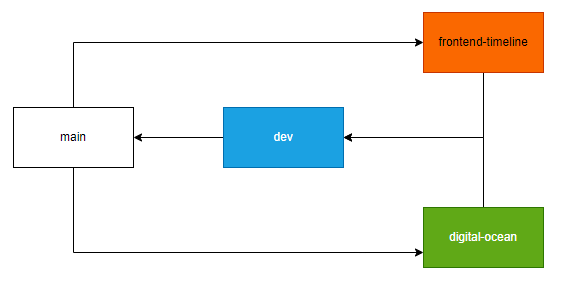
\includegraphics[width=0.7\linewidth]{report/images/branching.png}
    \caption{General branching strategy}
    \label{fig:gen_branch}
\end{figure}

\begin{figure}[H]
    \centering
    \captionsetup{justification=centering,margin=1cm}
    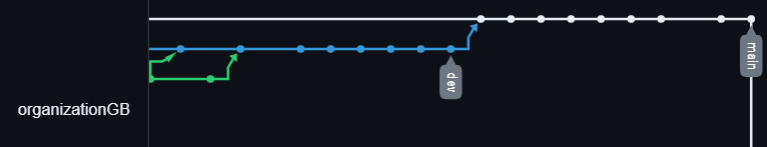
\includegraphics[width=0.7\linewidth]{report/images/git_branching.png}
    \caption{Example use of branching strategy}
    \label{fig:ex_branch}
\end{figure}

It can be seem that the temporary branches are derived from the main branch, and when the functionality is implemented, 
it is merged into the dev branch to be tested. 

\subsection{Development process and tools}
%https://dazzling-screen-208.notion.site/0d2059fc70b34671a8cd3f4f733d4909?v=0b5db8d8c829404e8ae96bb76ca5e6b7



\subsection{Monitoring}

\subsection{Logging}

\subsection{Security assessment}
From our security assessment we worked on blocking the risks with the highest likelihood. The first is \textit{An attacker could gain unauthorized access to the codebase}
- An attacker could easily find passwords and usernames in our public codebase. Now these are in github secrets such that an adversary cannot just 
find these at the public codebase. Another precaution would be to work with the risk \textit{Weak authentication and authorization mechanisms}
 - We are using default values such as postgres as username and password for the database. These should ofc be changed to something following the
 new security protocols standards. 

 \subsection{Scaling and load balancing}

 \subsection{AI-assistants}